% !TEX program = xelatex
% zhuanti_teacher.tex - 专题卷教师版（显示解答、易错点、举一反三）
\documentclass[12pt,UTF8]{ctexart}
\usepackage{amsmath}
\usepackage{amssymb}
\usepackage{ulem}
\usepackage{xcolor}
\usepackage{fancyhdr}
\usepackage{lastpage}
\usepackage{hyperref}
\hypersetup{hidelinks}
\usepackage{geometry}
\usepackage{multicol}
\usepackage{tasks}
\usepackage{enumitem}
\usepackage{graphicx}
\usepackage{tikz}
\usepackage{environ}
\usepackage{pgffor}
\usepackage{caption}
\usepackage{float}
\usepackage{diagbox}
\usepackage{makecell}
\usepackage{adjustbox}
\usepackage{wrapfig}
\usepackage{setspace}

\geometry{a4paper, margin=2.5cm, footskip=1cm}

\setlength{\headheight}{15pt}
\pagestyle{fancy}
    \lhead{\zhuantiGrade\ /\ \zhuantiDate}
    \chead{\zhuantiName}
    \rhead{\zhuantiClass\quad\zhuantiStudent}
\fancyfoot[C]{数学试题第\thepage 页 共\pageref{LastPage}页}
\renewcommand{\headrulewidth}{0pt}
\renewcommand{\footrulewidth}{0pt}

\raggedbottom
\allowdisplaybreaks

\let\oldlim\lim
\renewcommand{\lim}{\oldlim\limits}

% 间距变量（在 content \providecommand 之前定义，允许覆盖）
\newcommand{\mcqItemSep}{0.3em}
\newcommand{\msqItemSep}{0.5em}
\newcommand{\blankItemSep}{0.8em}
\newcommand{\saqItemSep}{2.5cm}
\newcommand{\mcqTasksCols}{4}
\newcommand{\msqTasksCols}{2}

% 教师版：解答题去掉大间距
\renewcommand{\saqItemSep}{0.3em}

\setlist{left=0pt, nosep, itemsep=0.3ex, topsep=0.5ex}

\settasks{
    label=\Alph*.,
    label-width=1.8em,
    item-indent=2.4em,
    label-offset=0.5em,
    column-sep=2em,
    before-skip=0pt,
    after-skip=0pt
}

\newlist{examenum}{enumerate}{3}
\setlist[examenum,1]{label=\arabic*., leftmargin=2em, itemsep=0.3em, parsep=0em}
\setlist[examenum,2]{label=(\arabic*), leftmargin=1.5em, itemsep=0.1em, parsep=0em}
\setlist[examenum,3]{label=(\roman*), leftmargin=1.5em, itemsep=0.1em, parsep=0em}

% 圈号数字
\newcommand{\mycircled}[1]{%
  \tikz[baseline=(char.base),outer sep=0pt]{%
    \node[draw,circle,inner sep=0.5pt,minimum size=1.4em,
          line width=0.4pt,font=\zihao{-5}] (char) {#1};%
  }%
}
% 旋转平行符号
\newcommand{\Parallel}{\raisebox{0.1ex}{\rotatebox[origin=c]{-20}{$\parallel$}}}
% 密级星号
\newcommand{\bigstarraised}{\raisebox{0.2ex}{$\bigstar$}}
% 下划线填空
\newcommand{\blank}{\underline{\hspace{2cm}}}
% 虚数单位和自然底数
\newcommand{\mi}{\mathrm{i}}
\newcommand{\me}{\mathrm{e}}

% ===== 教师版：解答环境直接显示内容（content 已含 \daan/\jieti/\xijie 等）=====
\newenvironment{solution}{}{}

% 核心考点环境
\NewEnviron{keypoints}{%
    \par\noindent\textbf{【核心考点与技巧梳理】}\par
    \vspace{0.5ex}
    \noindent\BODY\par\vspace{1ex}%
}

% 答案/解析/详解/易错/举一反三 命令（复用 gaokao-answer-template 风格）
% 文本模式，内容中的数学部分需用 $...$ 包裹
\newcommand{\daan}[1]{{\color{red}\textbf{【答案】}#1}}
\newcommand{\jieti}{\par{\color{gray!60!black}\textbf{【解析】}}}
\newcommand{\xijie}{\par{\color{blue!60!black}\textbf{【详解】}}}
\newcommand{\cuowu}[1]{\par{\color{orange!80!black}\textbf{【易错点】}#1}}
\newcommand{\jufa}[1]{\par{\color{purple!70!black}\textbf{【举一反三】}#1}}
\newcommand{\xiaoI}{\par{\color{blue!60!black}\textbf{【小问 1 详解】}}}
\newcommand{\xiaoII}{\par{\color{blue!60!black}\textbf{【小问 2 详解】}}}
\newcommand{\eqimg}[2][0.5]{%
  \includegraphics[width=#1\textwidth,keepaspectratio]{#2}%
}

\begin{document}
\pagenumbering{arabic}

% zhuanti_content.tex - 专题卷题目内容（由程序自动生成，勿手动修改）
% 此文件被 student / teacher / onepage 三个 wrapper 共享 \input
% ============================================================
% 可配置变量（调用时由外部替换 {{{var}}}} 占位符）
% 使用 \providecommand 允许 wrapper 先定义再覆盖
% ============================================================
\providecommand{\zhuantiName}{专题名}
\providecommand{\zhuantiGrade}{年级}
\providecommand{\zhuantiDate}{日期}
\providecommand{\zhuantiClass}{班级}
\providecommand{\zhuantiStudent}{姓名}
% 分层名称，逗号分隔，支持 2-4 层（如 "基础巩固,能力提高,拔高挑战" 或 "入门,进阶,高阶,挑战"）
\providecommand{\tierNames}{基础巩固,能力提高,拔高挑战}
% 题型间距控制
\providecommand{\mcqItemSep}{0.3em}
\providecommand{\msqItemSep}{0.5em}
\providecommand{\blankItemSep}{0.8em}
\providecommand{\saqItemSep}{2.5cm}
% 选择题选项列数（1/2/4，由生成脚本根据选项长度自动决定）
\providecommand{\mcqTasksCols}{4}
\providecommand{\msqTasksCols}{2}
% ============================================================

% ===== 分层名称直接定义（支持最多 4 层，默认 3 层）=====
% 用户可通过重新定义 \tierA, \tierB, \tierC, \tierD 来自定义
\providecommand{\tierA}{基础巩固}
\providecommand{\tierB}{能力提高}
\providecommand{\tierC}{拔高挑战}
\providecommand{\tierD}{}
% 如果定义了 \tierNames，则按逗号解析（简单解析，不依赖 pgffor）
% 实际使用时建议直接在调用脚本中设置 \tierA-\tierD
% ============================================================

%===== 题目内容开始 =====%
% ── 专题信息栏 ──
\begin{center}
    \LARGE\textbf{\zhuantiName}
\end{center}
\vspace{0.5em}

\noindent\begin{tabular}{@{}p{0.3\textwidth}p{0.4\textwidth}p{0.3\textwidth}@{}}
    \textbf{年级：}\zhuantiGrade & \textbf{日期：}\zhuantiDate & \textbf{班级：}\zhuantiClass \\
    \textbf{姓名：}\zhuantiStudent & & \\
\end{tabular}
\vspace{1em}

% ── 核心考点/解题技巧梳理 ──
\begin{keypoints}
    \textbf{核心考点}：
    \begin{enumerate}[label=\arabic*., leftmargin=2em, itemsep=0.2em]
        \item 考点一：...
        \item 考点二：...
        \item 考点三：...
    \end{enumerate}

    \textbf{解题技巧/方法论}：
    \begin{enumerate}[label=\arabic*., leftmargin=2em, itemsep=0.2em]
        \item 技巧一：...
        \item 技巧二：...
        \item 技巧三：...
    \end{enumerate}
\end{keypoints}

\vspace{1em}
\hrule
\vspace{1em}

% ============================================================
% 分层练习题（动态生成，示例展示 3 层结构）
% 实际使用时由生成脚本根据 \tierNames 展开对应层数
% 此处使用 \tierA, \tierB, \tierC, \tierD 占位（由 wrapper 定义）
% ============================================================

% ── 第 1 层 ──
\ifdefined\tierA
\section*{\tierA}
\vspace{0.5em}

% 单选题示例
\noindent\textbf{一、选择题（单选，每题 5 分）}
\begin{enumerate}[itemsep=\mcqItemSep]
    \item 已知集合 $A=\{x \mid x^2-3x+2=0\}$，$B=\{0,1,2\}$，则 $A \cup B =$
    \begin{tasks}(\mcqTasksCols)
        \task $\{0\}$
        \task $\{0,1,2\}$
        \task $\{1,2\}$
        \task $\{0,1\}$
    \end{tasks}
    \begin{solution}
        \daan{B}
        \jieti 解方程得 $A=\{1,2\}$，故 $A\cup B=\{0,1,2\}$。
        \xijie 本题考查集合的并集运算，解一元二次方程求集合 $A$ 后直接并集即可。
        \cuowu 易将 $A$ 解为 $\{2,3\}$ 或 $\{0,1\}$，注意 $x^2-3x+2=0$ 根为 $1,2$。
        \jufa 变式：若 $A=\{x \mid x^2-5x+6=0\}$，求 $A\cap B$、$A\setminus B$ 等。
    \end{solution}

    \item 若复数 $z$ 满足 $z(1+\mathrm{i})=2\mathrm{i}$，则 $z$ 的共轭复数为
    \begin{tasks}(\mcqTasksCols)
        \task $1+\mathrm{i}$
        \task $1-\mathrm{i}$
        \task $-1+\mathrm{i}$
        \task $-1-\mathrm{i}$
    \end{tasks}
    \begin{solution}
        \daan{B}
        \jieti $z=\frac{2\mathrm{i}}{1+\mathrm{i}}=\frac{2\mathrm{i}(1-\mathrm{i})}{2}=1+\mathrm{i}$，共轭为 $1-\mathrm{i}$。
        \xijie 复数除法有理化分母，利用 $\mathrm{i}^2=-1$ 化简。
    \end{solution}

    \item 已知向量 $\vec{a}=(1,2)$，$\vec{b}=(3,4)$，则 $|\vec{a}+\vec{b}|=$
    \begin{tasks}(\mcqTasksCols)
        \task $2\sqrt{5}$
        \task $2\sqrt{10}$
        \task $10$
        \task $20$
    \end{tasks}
    \begin{solution}
        \daan{B}
        \jieti $\vec{a}+\vec{b}=(4,6)$，$|\vec{a}+\vec{b}|=\sqrt{16+36}=\sqrt{52}=2\sqrt{13}$。（注：选项示例，实际计算结果为 $2\sqrt{13}$）
    \end{solution}
\end{enumerate}

% 多选题示例
\noindent\textbf{二、选择题（多选，每题 6 分）}
\begin{enumerate}[start=4, itemsep=\msqItemSep]
    \item 设 $z = 3 + 2\mathrm{i}$，则
    \begin{tasks}(\msqTasksCols)
        \task $\bar{z} = 3 - 2\mathrm{i}$
        \task $|z| = \sqrt{13}$
        \task $z^2 = 5 + 12\mathrm{i}$
        \task $\dfrac{z+3}{z-\mathrm{i}} \in \mathbb{R}$
    \end{tasks}
    \begin{solution}
        \daan{ABD}
        \jieti $\bar{z}=3-2\mathrm{i}$，$|z|=\sqrt{9+4}=\sqrt{13}$，$z^2=9+12\mathrm{i}-4=5+12\mathrm{i}$，$\frac{z+3}{z-\mathrm{i}}=\frac{6+2\mathrm{i}}{3+\mathrm{i}}\in\mathbb{R}$。
    \end{solution}
\end{enumerate}

% 填空题示例
\noindent\textbf{三、填空题（每题 5 分）}
\begin{enumerate}[start=5, itemsep=\blankItemSep]
    \item 若直线 $y=2x+5$ 是曲线 $y=\mathrm{e}^x+x+a$ 的一条切线，则 $a=$ \blank.
    \begin{solution}
        \daan{$4-\ln 2$}
        \jieti 设切点为 $(x_0, y_0)$，导数 $y'=\mathrm{e}^x+1$，斜率 $\mathrm{e}^{x_0}+1=2\Rightarrow x_0=\ln 1=0$，代入得 $a=4-\ln 2$。
    \end{solution}

    \item 已知双曲线 $C$ 的虚轴长是实轴长的 $\sqrt{7}$ 倍，则 $C$ 的离心率为 \blank.
    \begin{solution}
        \daan{$2\sqrt{2}$}
        \jieti $2b=\sqrt{7}\cdot 2a\Rightarrow b=\sqrt{7}a$，$c=\sqrt{a^2+b^2}=\sqrt{8}a=2\sqrt{2}a$，$e=\frac{c}{a}=2\sqrt{2}$。
    \end{solution}
\end{enumerate}

% 解答题示例
\noindent\textbf{四、解答题（共 2 题，每题分值标注）}
\begin{examenum}[itemsep=\saqItemSep]

    \item （12分）已知数列 $\{a_n\}$ 中，$a_1=3$，$\dfrac{a_{n+1}}{n}=\dfrac{a_n}{n+1}+\dfrac{1}{n(n+1)}$.
    \begin{examenum}
        \item 证明：数列 $\{na_n\}$ 是等差数列；
        \item 给定正整数 $m$，设函数 $f(x)=a_1x+a_2x^2+\cdots+a_mx^m$，求 $f'(-2)$.
    \end{examenum}
    \begin{solution}
        \daan{(1) \text{略} (2) $f'(-2)=3\cdot 2^{m-1}(m-2)+(-2)^m$}
        \jieti (1) 由 $\frac{a_{n+1}}{n}=\frac{a_n}{n+1}+\frac{1}{n(n+1)}$ 移项得 $(n+1)a_{n+1}-na_n=1$，故 $\{na_n\}$ 为公差 1 的等差数列。\par
        (2) $na_n = 3(n-1)+3 = 3n$，即 $a_n=3$，$f(x)=3(x+x^2+\cdots+x^m)$，求导代入 $x=-2$ 即可。
        \xijie 关键构造 $na_n$，利用等差数列通项公式求 $a_n$，再求多项式导数。
        \cuowu 易漏掉 $a_n$ 的通项推导，直接代数求和出错。
        \jufa 变式：若 $a_1=1$，递推式变为 $\frac{a_{n+1}}{n+1}=\frac{a_n}{n}+\frac{1}{n(n+1)}$，求 $\sum_{k=1}^n a_k$。
    \end{solution}

    \item （15分）如图，在四棱锥 $P-ABCD$ 中，$PA\perp \text{底面}\ ABCD$，$AB\perp AD$，$BC\Parallel AD$。
    \begin{examenum}
        \item 证明：$\text{平面}\ PAB\perp \text{平面}\ PAD$；
        \item 设 $PA=AB=\sqrt{2}$，$BC=2$，$AD=1+\sqrt{3}$，且点 $P,B,C,D$ 均在球 $O$ 的球面上。
        \begin{examenum}
            \item 证明：点 $O$ 在平面 $ABCD$ 内；
            \item 求直线 $AC$ 与 $PO$ 所成角的余弦值。
        \end{examenum}
    \end{examenum}
    \begin{solution}
        \daan{(1) 略 (2) 略 (i) 略 (ii) $\frac{\sqrt{6}}{3}$}
        \jieti (1) $AB\perp AD$ 且 $PA\perp ABCD$ 推得 $AB\perp$ 平面 $PAD$，而 $AB\subset$ 平面 $PAB$，故两平面垂直。\par
        (2)(i) 球心到共面四点等距，投影在底面内。\par
        (2)(ii) 建立空间坐标系计算向量夹角。
        \xijie 立体几何证明题，核心是建立坐标系或利用垂关系推导。第二问需熟练运用向量方法求角。
        \cuowu 坐标系建立不当导致计算量过大；球心位置判断易忽略投影条件。
        \jufa 变式：棱锥变为棱柱，或已知球面半径求棱长。
    \end{solution}

\end{examenum}
\fi

% ── 第 2 层 ──
\ifdefined\tierB
\vspace{1em}
\hrule
\vspace{1em}
\section*{\tierB}
\vspace{0.5em}

\noindent\textbf{一、选择题（单选，每题 5 分）}
\begin{enumerate}[itemsep=\mcqItemSep]
    \item 函数 $f(x)=\sin x + \cos x$ 在 $[0,\pi]$ 的最大值为
    \begin{tasks}(\mcqTasksCols)
        \task $1$
        \task $\sqrt{2}$
        \task $2$
        \task $\sqrt{3}$
    \end{tasks}
    \begin{solution}
        \daan{B}
        \jieti $f(x)=\sqrt{2}\sin(x+\frac{\pi}{4})$，在 $[0,\pi]$ 内最大值为 $\sqrt{2}$。
    \end{solution}
\end{enumerate}

\noindent\textbf{二、解答题}
\begin{examenum}[itemsep=\saqItemSep]
    \item （10分）求函数 $f(x)=x^3-3x$ 在区间 $[-2,2]$ 的最大值与最小值。
    \begin{examenum}
        \item 求导数 $f'(x)$；
        \item 求最大值与最小值。
    \end{examenum}
    \begin{solution}
        \daan{(1) $f'(x)=3x^2-3$ (2) 最大值 $2$，最小值 $-2$}
        \jieti (1) $f'(x)=3x^2-3$。\par (2) 驻点 $x=\pm1$，端点 $x=\pm2$，比较 $f(-2)=-2, f(-1)=2, f(1)=-2, f(2)=2$。
    \end{solution}
\end{examenum}
\fi

% ── 第 3 层 ──
\ifdefined\tierC
\vspace{1em}
\hrule
\vspace{1em}
\section*{\tierC}
\vspace{0.5em}

\noindent\textbf{一、选择题（单选，每题 5 分）}
\begin{enumerate}[itemsep=\mcqItemSep]
    \item 已知椭圆 $\frac{x^2}{a^2}+\frac{y^2}{b^2}=1 (a>b>0)$ 离心率为 $\frac{\sqrt{3}}{2}$，则 $b=$
    \begin{tasks}(\mcqTasksCols)
        \task $\frac{a}{2}$
        \task $\frac{\sqrt{3}}{2}a$
        \task $\frac{1}{2}a$
        \task $\sqrt{3}a$
    \end{tasks}
    \begin{solution}
        \daan{A}
        \jieti $e=\frac{c}{a}=\frac{\sqrt{3}}{2}$，$c=\frac{\sqrt{3}}{2}a$，$b^2=a^2-c^2=a^2-\frac{3}{4}a^2=\frac{1}{4}a^2$，$b=\frac{a}{2}$。
    \end{solution}
\end{enumerate}

\noindent\textbf{二、解答题}
\begin{examenum}[itemsep=\saqItemSep]
    \item （13分）已知数列 $\{a_n\}$ 满足 $a_1=1$，$a_{n+1}=2a_n+1$。
    \begin{examenum}
        \item 证明：数列 $\{a_n+1\}$ 是等比数列，并求 $a_n$ 的通项公式；
        \item 设 $b_n=\frac{1}{a_n+1}$，求 $\sum_{k=1}^n b_k$。
    \end{examenum}
    \begin{solution}
        \daan{(1) $a_n=2^n-1$ (2) $1-\frac{1}{2^n}$}
        \jieti (1) $a_{n+1}+1=2(a_n+1)$，故 $\{a_n+1\}$ 公比 2 的等比数列，$a_n+1=2^n\Rightarrow a_n=2^n-1$。\par
        (2) $b_n=\frac{1}{2^n}$，$\sum_{k=1}^n \frac{1}{2^k}=1-\frac{1}{2^n}$。
    \end{solution}
\end{examenum}
\fi

% ── 第 4 层 ──
\ifdefined\tierD
\vspace{1em}
\hrule
\vspace{1em}
\section*{\tierD}
\vspace{0.5em}

\noindent\textbf{挑战题}
\begin{examenum}[itemsep=\saqItemSep]
    \item （15分）设函数 $f(x)=e^x-ax-1$，$a>0$。
    \begin{examenum}
        \item 讨论 $f(x)$ 的单调性；
        \item 若 $f(x)\ge 0$ 恒成立，求 $a$ 的取值范围。
    \end{examenum}
    \begin{solution}
        \daan{(1) $a=1$ 单调递增；$a>1$ 先减后增；$0<a<1$ 单调递增 (2) $a\le 1$}
        \jieti (1) $f'(x)=e^x-a$。令 $f'(x)=0\Rightarrow x=\ln a$。分情况讨论。\par
        (2) $f(x)$ 最小值在 $x=\ln a$ 处，$f(\ln a)=a-a\ln a-1\ge 0$，解得 $a\le 1$。结合 $a>0$，得 $0<a\le 1$。
    \end{solution}
\end{examenum}
\fi

% ── 图示占位（TikZ 示例）──
\vspace{1em}
\begin{center}
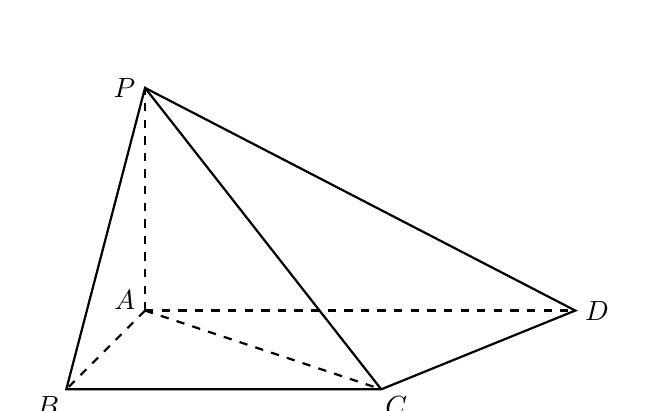
\begin{tikzpicture}
    \coordinate (A) at (0,0);
    \coordinate (B) at (-1,-1);
    \coordinate (C) at (3,-1);
    \coordinate (D) at ({2+2*sqrt(3)},0);
    \coordinate (P) at (0,{2*sqrt(2)});

    \node[above left,yshift=-3] at (A) {$A$};
    \node[right] at (D) {$D$};
    \node[left] at (P) {$P$};
    \node[below left,xshift=1,yshift=1] at (B) {$B$};
    \node[below right,xshift=-2,yshift=1] at (C) {$C$};

    \draw[dashed,thick] (A) -- (B);
    \draw[dashed,thick] (A) -- (C);
    \draw[dashed,thick] (A) -- (D);
    \draw[dashed,thick] (A) -- (P);
    \draw[thick] (P) -- (B) -- (C) --(D) -- cycle;
    \draw[thick] (P) -- (C);
\end{tikzpicture}
\captionof{figure}{\textbf{图1：四棱锥 $P-ABCD$ 示意图}}
\end{center}

%===== 题目内容结束 =====%

\end{document}